%%
%% This is file `sample-sigconf.tex',
%% generated with the docstrip utility.
%%
%% The original source files were:
%%
%% samples.dtx  (with options: `sigconf')
%% 
%% IMPORTANT NOTICE:
%% 
%% For the copyright see the source file.
%% 
%% Any modified versions of this file must be renamed
%% with new filenames distinct from sample-sigconf.tex.
%% 
%% For distribution of the original source see the terms
%% for copying and modification in the file samples.dtx.
%% 
%% This generated file may be distributed as long as the
%% original source files, as listed above, are part of the
%% same distribution. (The sources need not necessarily be
%% in the same archive or directory.)
%%
%% The first command in your LaTeX source must be the \documentclass command.
\documentclass[sigconf]{acmart}
\usepackage{multirow, tabularx, subcaption, float}
%% NOTE that a single column version may be required for 
%% submission and peer review. This can be done by changing
%% the \doucmentclass[...]{acmart} in this template to 
%% \documentclass[manuscript,screen]{acmart}
%% 
%% To ensure 100% compatibility, please check the white list of
%% approved LaTeX packages to be used with the Master Article Template at
%% https://www.acm.org/publications/taps/whitelist-of-latex-packages 
%% before creating your document. The white list page provides 
%% information on how to submit additional LaTeX packages for 
%% review and adoption.
%% Fonts used in the template cannot be substituted; margin 
%% adjustments are not allowed.
%%
%%
%% \BibTeX command to typeset BibTeX logo in the docs
\AtBeginDocument{%
  \providecommand\BibTeX{{%
    \normalfont B\kern-0.5em{\scshape i\kern-0.25em b}\kern-0.8em\TeX}}}

%% Rights management information.  This information is sent to you
%% when you complete the rights form.  These commands have SAMPLE
%% values in them; it is your responsibility as an author to replace
%% the commands and values with those provided to you when you
%% complete the rights form.
\setcopyright{acmcopyright}
\copyrightyear{2018}
\acmYear{2021}
\acmDOI{10.1145/1122445.1122456}

%% These commands are for a PROCEEDINGS abstract or paper.
\acmConference[Woodstock '18]{Woodstock '18: ACM Symposium on Neural
  Gaze Detection}{June 03--05, 2018}{Woodstock, NY}
\acmBooktitle{Woodstock '18: ACM Symposium on Neural Gaze Detection,
  June 03--05, 2018, Woodstock, NY}
\acmPrice{15.00}
\acmISBN{978-1-4503-XXXX-X/18/06}


%%
%% Submission ID.
%% Use this when submitting an article to a sponsored event. You'll
%% receive a unique submission ID from the organizers
%% of the event, and this ID should be used as the parameter to this command.
%%\acmSubmissionID{123-A56-BU3}

%%
%% The majority of ACM publications use numbered citations and
%% references.  The command \citestyle{authoryear} switches to the
%% "author year" style.
%%
%% If you are preparing content for an event
%% sponsored by ACM SIGGRAPH, you must use the "author year" style of
%% citations and references.
%% Uncommenting
%% the next command will enable that style.
%%\citestyle{acmauthoryear}

%%
%% end of the preamble, start of the body of the document source.
\begin{document}

%%
\title{Facial Expression Recognition for Cloud Robotics}

%%
%% The "author" command and its associated commands are used to define
%% the authors and their affiliations.
%% Of note is the shared affiliation of the first two authors, and the
%% "authornote" and "authornotemark" commands
%% used to denote shared contribution to the research.
\author{Charlie Maclean}
\affiliation{%
  \institution{University of Cambridge}
  \city{Cambridge}
  \country{United Kingdom}
}
\email{cm927@cam.ac.uk}


%%
%% By default, the full list of authors will be used in the page
%% headers. Often, this list is too long, and will overlap
%% other information printed in the page headers. This command allows
%% the author to define a more concise list
%% of authors' names for this purpose.
\renewcommand{\shortauthors}{Charlie Maclean}

\begin{abstract}

As social robots become widespread, it will be essential that they can
classify the emotions of humans around them, in order to interact in a
meaningful and helpful way. But limited hardware means they
may have to offload video data to the cloud, reducing the resolution of the
content. This work focuses on evaluating the fitness of neural network models
for cloud computing, specifically the effect of changing spatial and temporal 
resolution on the
classification of emotion in video. I built different models to assess each
models performance when given lower resolution video. The results show that by
applying a CNN-LSTM model to an 8-class classification problem, we can achieve 81\% accuracy on high resolution
video, and maintain 76\% accuracy even at the lowest resolution. To the best of
my knowledge this is the first work that investigates the effect of changing
both spatial and temporal resolution on video-based sentiment classification.

\end{abstract}


\keywords{Affective computing, robotics, cloud computing, emotions, arousal, valence, resolution.}

%%
%% This command processes the author and affiliation and title
%% information and builds the first part of the formatted document.
\maketitle

\section{Introduction}

\begin{figure}
  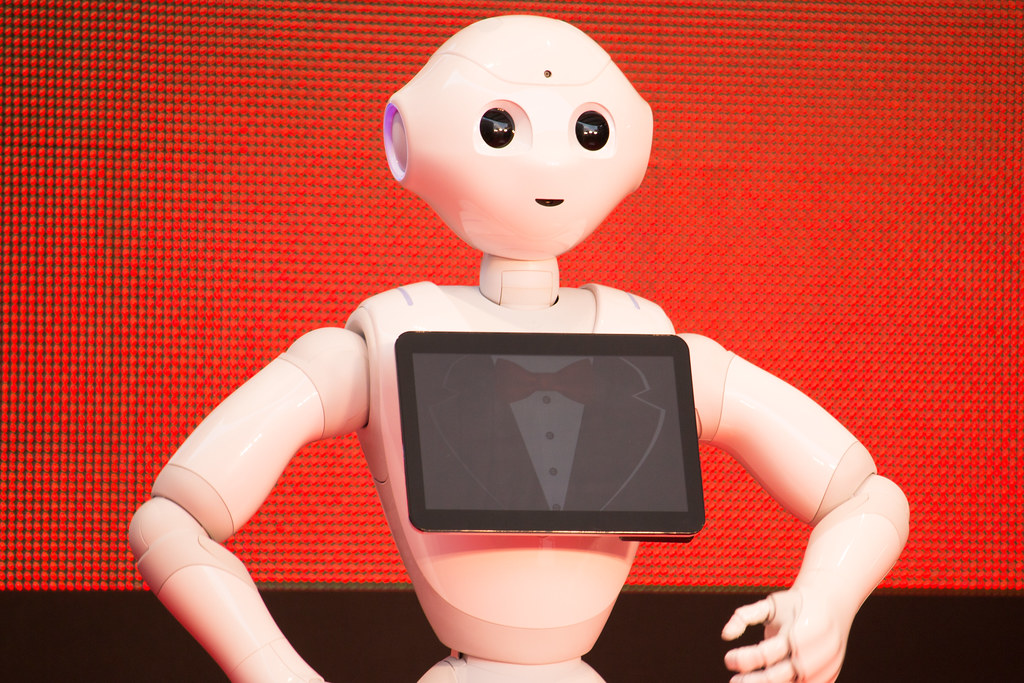
\includegraphics[width=\linewidth]{care-robot.jpg}
  \caption{Pepper by SoftBank Robotics, an example of a social robotic
  platform which has been trialled in care homes in the UK. Photograph by Dick
  Thomas, via creative commons
  (\href{https://search.creativecommons.org/photos/e802da62-8b2f-4f10-9520-bb6c5a0e03db}{source}).}
  \label{fig:pepper}
\end{figure}

Social robots are becoming increasingly widespread, with uses in a wide range
of locations, providing help in hospitals \cite{moxi}, care homes \cite{ElliQ}
and schools \cite{AV1}. These robots are frequently required to
interact meaningfully with humans, and in order to do so it is essential that
they are able to classify emotions so they can react accordingly. However, many social robotic
platforms lack the computational hardware required to perform classification
\cite{celiktutan18}.
Hence, it will likely be necessary to move to a cloud robotic framework,
where sensing data is offloaded to the cloud and processed there. Unreliable
network conditions mean we must be prepared for video data to enter the cloud
at reduced spatial and temporal resolutions. 

In past years, neural networks have become ubiquitous for classifying emotion,
due to their ability to learn patterns that are extremely difficult to
hard-code.
However they can suffer from not being generalizable, especially if a network
is trained in one domain, then deployed in another. For example, a network
trained on high resolution data may well be less effective at classifying low
resolution data. 

For classifying images, there is a large volume of work looking at using
convolutional neural networks (CNNs). When applied to an image, a CNN
convolves a filter with the pixel data, hopefully generating meaningful features. 
CNNs have found widespread use across various domains, including facial
recognition \cite{lawrence1997face}, object detection and object classification
\cite{szegedy2014going}.
Several architectures have been proposed offering impressive ability to learn
features from images, for example the VGG16 network \cite{simonyan2014very} and the
ResNet50 network \cite{he2016deep}, both of which were able to achieve winning results in
the ImageNet object detection and classification challenge \cite{ILSVRC15}.

For classifying videos, it is often vital to take temporal data into account,
and as a result Recurrent Neural Networks (RNNs) \cite{rumelhart1985learning} are a good
choice. RNNs have some internal state, or memory, which they use to process
sequences, learning patterns that may vary over time. A very popular
architecture is Long Short Term Memory \cite{hochreiter1997long} {(LSTM),
which makes use of gates to
control the flow into and out of cells in the architecture. LSTMs have found
wide usage, across speech recognition \cite{graves2005framewise}, market prediction
\cite{islam2020foreign} and handwriting recognition \cite{graves2008unconstrained}.

In this work we create a number of classifiers which are tested on video at a
variety of resolutions and frame rates, in order to deduce which classifiers
may be useful for cloud robotics. The classifiers are tested on the 8-class
RAVDESS emotional
video dataset \cite{livingstone2018ryerson}, and our results show that we can
achieve an accuracy of 81 \% on high resolution video, while maintaining 76\%
accuracy on the lowest resolution video.

The rest of the paper is structured as follows: Section 2 gives an overview of
previous work on similar problems, Section 3 gives details about the
methodology employed in the study. Then, Section 4 discusses the results
before Section 5 goes over future research directions. Finally, Section 6
concludes the paper with an overview of the findings. 

\section{Related Work}

In this section I give an overview of prior work on facial expression recognition
techniques, first for images, and then for videos, followed by a section 
on other studies that have looked at classifying data at reduced resolutions. 

\subsection{Facial Expression Recognition in Images}

Facial expressions have always been a useful mechanism allowing people to 
communicate their emotions between
each other. There has been a large volume of research into the
mechanisms which allow this non-verbal communication to happen. An early work
by P. Ekman and W.V. Friesen introduced the Facial Action Coding System
(FACS) \cite{friesen1978facial}, which described a list of facial action units
- regions which change as a person changes their expression. The work further describes
how a given facial expression could be described as a combination of action
units. Following this work, P. Ekman et al. detailed how a mapping can be made
between those facial action units and a person's emotions
\cite{ekman1997face}, a work which inspired the use of machines to detect
emotions. 
I will now detail the work that has been put into this field, 
splitting the research into those that make use of deep
networks, and those before deep networks became widespread. 

Before the use of deep networks, there were two main approaches to sentiment
classification for images - rule-based methods, and appearance based methods.
First, the rule-based methods were centred around detecting facial action
units individually, and then piecing together the results from the facial
action unit regions to derive an overall emotion, for example in Y. Tian
et al.'s work \cite{tian2001recognizing}. However such techniques
suffered as recognizing an individual action unit is not an easy task. In the
alternative approach, appearance based methods, some features are extracted
from the overall face, and then those features are passed through a machine
learning classifier. For example, M.S. Bartlett et al. found that they could
achieve good results by extracting features using Gabor filters, followed by a
Support Vector Machine (SVM) \cite{bartlett2005recognizing}. Additionally, J.
Whitehall and C. Omlin showed that comparable results could be obtained in
significantly quicker time by using Haar wavelets to obtain features
before passing through a SVM \cite{whitehill2006haar}. 

In the previously mentioned techniques, processing of emotions had been split into learning
features, selecting features and then using a classifier to learn the
patterns within those features. The downside of taking that approach is that the first layers do not
get feedback from the latter layers. Deep learning aims to solve that, by
integrating the feature finding, selection and classification into one deep
network that can be trained at once. One of the early papers making use of
this technique was by P. Liu et al. \cite{liu2014facial}, who suggested using
a Boosted Deep Belief Network. This network consisted of several deep networks
learning features, and some of these networks get boosted based on their
performance. Also,  Liu et al. introduced CNNs to the 
problem, with their CNN Ensemble network\cite{liu2016facial}. The network consisted of three 
different convolutional networks, which proved to achieve better results than
a single CNN.

\subsection{Facial Expression Recognition in Videos}

When classifying emotion in videos, there is additional information that can
be extracted by recognising the way the face changes over time. There are
several papers which attempt to do this, which I will now go over, beginning
with aggregation techniques. Aggregation techniques classify each frame within
a video, and then combine the results with an aggregator. In
\cite{kahou2016emonets} and \cite{kahou2013combining}, S. Kahou et al. split
the video into 10 sections, and within each section aggregate the frame
predictions by taking the mean. They go on to use a SVM to classify using all 10
aggregate predictions. An alternative method was introduced in 
\cite{liu2014combining} where
M. Liu et al. showed that features from individual frames could be mapped to 
probabilistic distributions such as Gaussian distributions, which could then
be passed through a SVM.

An alternative approach focused on attempts to classify the level of
emotional intensity present in an individual frame - the idea being that you
could derive the emotion of a video by finding the frames with the strongest
emotions and just classifying those. 
In \cite{zhao2016peak} X. Zhao et al. propose a network which minimizes the differences
between an emotion at low intensity and the same emotion at high intensity, as
a way to get better classification of low intensity emotion. The downside of
their technique was that it required a training set consisting of pairs of the
same emotions at different intensities. To address this, 
in \cite{chen2018deep} J. Chen et al. used unsupervised clustering and a semisupervised 
SVM to detect peak and neutral frames in a large dataset.

Finally, deep spatio-temporal networks were introduced which use sequences of
frames as inputs to the networks, in the anticipation that we can learn more
information from the temporal dynamics of the images. C3Ds
\cite{tran2015learning} are the natural generalization of a CNN to 3
dimensions - instead of convolving an image with a 2D kernel, we convolve a
sequence of frames with a 3D kernel. These 3D techniques have been brought to
video emotion recognition, for example by X. Ouyang in \cite{ouyang2017audio}.
An alternative approach was taken in \cite{kim2017multi} where D. Kim et al.
tracked facial landmarks to generate trajectories which were used as features.
Finally, a common approach is to use a CNN to learn spatial features of an
image followed by a LSTM to learn the temporal features of the overall video,
as in D. Kim et al.'s work \cite{kim2017multiobjective}.

\subsection{Reduced resolution classification}

There have been some studies looking at how to cope when the face that
needs to be classified is at a low resolution. Firstly, Y. Tian
\cite{tian2004evaluation} looked at how low spatial resolution would affect
three steps in a facial expression analysis pipeline: face acquisition,
facial data extraction and finally expression recognition. Also, R. Khan et
al. produced a framework for expression recognition on low-resolution images
\cite{khan2013framework}, by suggesting a new set of features which work on
low resolution images - called a pyramid of local binary patterns. Finally, T.
Vo et al. proposed the pyramid with super resolution architecture
\cite{vo2020pyramid}, which made use of super resolution networks in order to
scale up low resolution images with minimal artefacts. 



\section{Methodology}
On this work I decided to start by training CNNs to classify individual
images, and then to see how I could use that trained CNN to classify multiple
frames within a video. I took this approach as it is logical to start with a
strong image classifier to build on for video classification.
The overall goal of this section is to build to a classifier which we can use to test
video at multiple spatial and temporal resolutions. We first introduce the
datasets used in the work, then discuss the image classifiers produced, before
finally talking about the techniques used to classify the videos.

\subsection{Datasets}

For learning facial expressions in images I used the FER+ dataset
\cite{barsoum2016training} from E. Barsoum et al., a large collection of
images first introduced as part of the FER-2013 dataset \cite{goodfellow2013challenges}.
The FER-2013 dataset consists of 36,685 48x48 greyscale images obtained
by searching for different emotions on Google Images. The dataset is split
into 7 categories - angry, sad, disgust, fear, happy, surprise and neutral.
FER+ uses the same collection of images as in FER-2013, but updated the labels
to be more accurate by crowd-sourcing the labelling and getting 10 taggers to
label each image. In this work, we use majority voting to decide the ground
truth of the images, discarding those for which there is no majority. 

To learn facial expressions in videos, I used the RAVDESS
\cite{livingstone2018ryerson} dataset by SR. Livingstone and FA. Russo. The
dataset consists of 24 professional actors speaking two different statements
while expressing one of eight emotions. The emotions include calm, happy, sad,
angry, fearful, surprise, disgust and neutral. The data is provided at 720p,
30 fps with a blank background, in laboratory settings.

To pre-process the video data, we crop the images to a box around the face. In
order to detect the bounding box around the face, we make use of Haar
cascades. The purpose of this study is not to focus on how to detect faces at
a reduced resolution as there is sufficient work already on that topic
(\cite{zheng2010face}, \cite{tian2004evaluation}).

\subsection{Training Image Recognition}

I used a ResNet50 CNN architecture which is a 50 layer member of the 
family of Residual Networks, designed by K.
He et al. \cite{DBLP:journals/corr/HeZRS15}. They were designed to tackle
image recognition tasks, and were significantly deeper than previously
introduced architectures, which allowed them to gain accuracy in several
recognition tasks. 
Further, despite the increase in depth, they managed to make
the networks relatively easy to optimize.

Instead of training the network beginning with random parameters, I made use
of transfer learning - where you use network weights obtained from a different
dataset/task. This helps to bootstrap the network, giving it a good place to start
learning the task you want.  
We use two different base models, which are publicly available - the first is
trained on ImageNet \cite{ILSVRC15}, a massive dataset of over a million
images, sorted into various nouns. Also, we use weights trained on the VGG
Face dataset \cite{parkhi2015deep}, which consists of 9,131 images of
different people's faces.
To train, I take the top layers off the pre-trained network, and then add two
dense layers to perform the classification on my task. I freeze the original
base of the network and train just the new top of the network. After this is
complete, I unfreeze the network and train the entirety of the network.

To train the network we use stochastic gradient descent, and in order to
obtain good hyperparameters  we use Bayesian optimization \cite{snoek2012practical}. Bayesian
optimization represents the problem as a Guassian process, which maps
hyperparameters to the optimization criteria. By doing this, it can focus the
hyperparameter search on those regions which are most likely to lead to good
results.

\subsection{Training Video Recognition}

To classify video, I decided to make use of the best network I previously used
for classifying images, with the logic that the patterns learnt there would be
applicable in the video domain too. In order to extend the network that was
designed for single images to video, with several image frames, I made use of 3
different techniques. The first two are quite simplistic - I classify each
frame of the video before then taking an aggregate of those results. For the
first technique, this aggregate is a mean of all the classification scores.
The second technique is where I take the max class for each frame, and then
take the mode of these classifications.

The third technique I used was a LSTM network, appended to the output of the
ResNet, to form a CNN-LSTM architecture. 
A whole video is fed into the network, and each frame then passes through the
ResNet to extract relevant features, which are then passed to the LSTM.
I used a LSTM with 1024 units, which
means the LSTM outputs 1024 different features. I follwed the LSTM with two
dense layers for the final classifcation.
I freeze the ResNet layers, so we just learn the temporal dynamics using the
lSTM. It was trained using the Adam
optimizer \cite{kingma2014adam}, which promises to be well suited for
optimization problems with a large number of parameters and data. 

To preprocess the video, I created copies of the video at 3 different
resolution and 3 different frame rates, for a total of 9 different clips for
each input. The resolutions and frame rates were chosen such that they give a
wide range of what may be possible over the internet. For resolutions, we had
720p (1280x720 px), 360p (480x360 px) and 144p (256x144 px), and for
frame rates we had 30 fps, 15 fps and 5 fps. 720p at 30 fps is feasible
with a fast internet connection, and low proximity to the server, and 144p at
5 fps would happen with a poor internet connection and/or large distance from
a server. 

\section{Evaluation}

In this section I walk through the results of the experiments, starting with
the image recognition task and then moving on to the video recognition tasks.

\subsection{Image Recognition}

\begin{table*}[htbp]
\caption{Classification results on the test set of the FER+ dataset.}
\label{tab:imageres}
\begin{tabular}{lccccccccccccccc}
\multirow{2}{*}{model} & \multicolumn{2}{c}{anger} &
\multicolumn{2}{c}{disgust} & \multicolumn{2}{c}{fear} &
\multicolumn{2}{c}{happiness} & \multicolumn{2}{c}{neutral} &
\multicolumn{2}{c}{sadness} & \multicolumn{2}{c}{surprise}  & Overall\\ \cline{2-16}
                       & Recall        & F1        
		       & Recall        & F1        & Recall        & F1
		       &  Recall        & F1        &  Recall        & F1
		       & Recall        & F1        & Recall        & F1    &
		       Accuracy    \\ \hline
RN50 on VGG & \textbf{0.86} &\textbf{0.85} &\textbf{0.33} &\textbf{0.45} &\textbf{0.49} &\textbf{0.58} &\textbf{0.95} &\textbf{0.94} &\textbf{0.65} &\textbf{0.71} &\textbf{0.85} &\textbf{0.86} &\textbf{0.91} &\textbf{0.88} &\textbf{0.86} \\
RN50 on ImageNet   & 0.63 &0.67 &0 &0 &0.21 &0.34 &0.89 &0.88 &0.44 &0.53 &0.81 &0.8 &0.9 &0.82 &0.78 \\
\end{tabular}
\end{table*}

In our image recognition task, I trained a ResNet50 network on the 7-class FER+
dataset, using transfer learning, with two different starting points. One
network was pre-trained on the ImageNet dataset, and one on the VGG Face
dataset. The recall and F1 score for each class, along with the overall
accuracy are plotted in Table \ref{tab:imageres}. The table clearly
demonstrates that the VGG pre-train outperforms ImageNet in each class, which
is likely due to the fact that VGG model had been trained to recognize specific facial
features, whereas ImageNet model is trained on a much wider set of objects so is
less dedicated to recognizing faces.

One area where both models underperform is in classifying disgust. This is largely
due to the fact that the FER+ dataset is quite unbalanced, with very few
disgust expressions within. Furthermore, the line between disgust and anger is
quite small, meaning that 47\% of the disgust images are labelled as
anger,
as can be seen in the confusion matrix in Figure \ref{fig:image-vgg}. There
are a couple of ways to address this in future, for example I could utilize a
weighted loss function which gives more weight to the minority
classes. Also I could use under-sampling of majority classes and over-sampling
for minority classes. Finally, I could use a Generative
Adversarial Network to generate more artificial faces for the minority
classes. However, I did not employ these techniques in this work, as my focus
was on classifying videos.

\begin{figure}[htbp]
	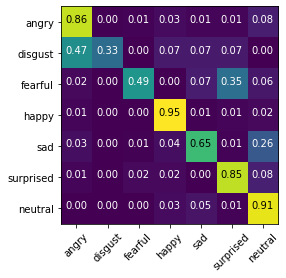
\includegraphics[width=0.7\linewidth]{images/image-vgg.png}
	\caption{Confusion matrix for ResNet50 pre-trained on VGG Face Dataset.}
  \label{fig:image-vgg}
\end{figure}




%%\begin{figure*} \caption{Congusion matrices for the ResNet50 models, based on the test
%%	set of the FER+ dataset.}
%%	\centering
%%  \hfill
%% \begin{subfigure}[b]{0.3\textwidth}
%%	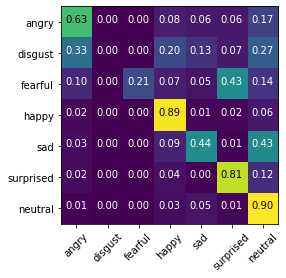
\includegraphics[width=\textwidth]{images/image-imagenet.png}
%%	\caption{ResNet50 pre-trained on ImageNet.}
%%  \label{fig:image-imagenet}
%%\end{subfigure}
%%\hfill
%%\begin{subfigure}[b]{0.3\textwidth}
%%	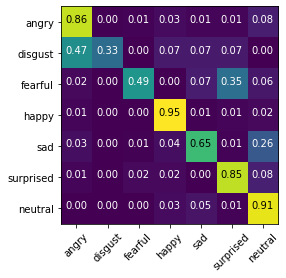
\includegraphics[width=\textwidth]{images/image-vgg.png}
%%	\caption{ResNet50 pre-trained on VGG Face Dataset.}
%%  \label{fig:image-vgg}
%%  \end{subfigure}
%%  \hfill
%%\end{figure*}

\subsection{Video Recognition}

\begin{figure*}[h]
	\centering
	\begin{subfigure}[b]{0.3\textwidth}
		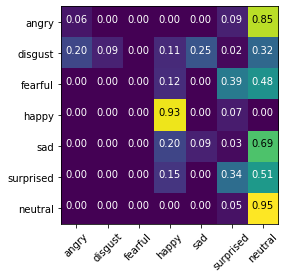
\includegraphics[width=\textwidth]{images/video-mean.png}
		\caption{Mean Classification}
		  \label{fig:video-mean}
	\end{subfigure}
	\hfill
	\begin{subfigure}[b]{0.3\textwidth}
		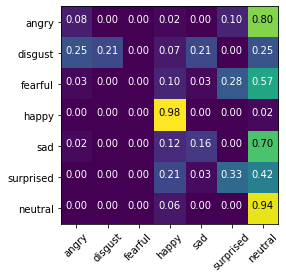
\includegraphics[width=\textwidth]{images/video-mode.png}
		\caption{Mode Classification}
		\label{fig:video-mode}
	\end{subfigure}
	\hfill
	\begin{subfigure}[b]{0.3\textwidth}
		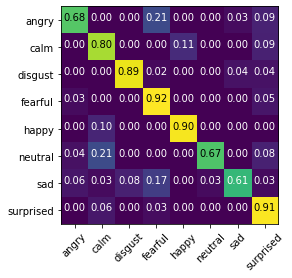
\includegraphics[width=\textwidth]{images/video-lstm.png}
		\caption{LSTM Classification}
		\label{fig:video-lstm}
	\end{subfigure}
	\caption{Confusion matrices for video classification on the RAVDESS dataset, based on the best results for any fps/resolution.}
	\label{fig:video}
\end{figure*}


\begin{table*}[h]
	\caption{Comparison of video classifiers accuracy on the RAVDESS dataset.}
	\label{tab:video}
	\begin{subtable}[b]{0.3\textwidth}
		\caption{Mean Classification}\label{tab:acc-mean}
		\begin{tabularx}{0.9\textwidth}{l X X X}
		&\multicolumn{3}{c}{Frame rate (fps)} \\\cmidrule{2-4}
		Resolution (px) &30 &15 &5 \\\cmidrule{1-4}
		1280x720 &0.26 &0.31 &0.30 \\
		640x360 &\textbf{0.33} &0.30 &0.28 \\
		256x144 &\textbf{0.33} &0.29 &0.31 \\
		\end{tabularx}
	\end{subtable}
	\begin{subtable}[b]{0.3\textwidth}
		\caption{Mode Classification}\label{tab:acc-mode}
		\begin{tabularx}{0.9\textwidth}{l X X X}
		&\multicolumn{3}{c}{Frame rate (fps)} \\\cmidrule{2-4}
		Resolution (px) &30 &15 &5 \\\cmidrule{1-4}
		1280x720 &0.27 &0.31 &0.31 \\
		640x360 &0.32 &0.30 &0.30 \\
		256x144 &\textbf{0.33} &0.31 &0.32 \\
		\end{tabularx}
	\end{subtable}
	\begin{subtable}[b]{0.3\textwidth}
		\caption{LSTM Classification}\label{tab:acc-lstm}
		\begin{tabularx}{0.9\textwidth}{l X X X}
		&\multicolumn{3}{c}{Frame rate (fps)} \\\cmidrule{2-4}
		Resolution (px) &30 &15 &5 \\\cmidrule{1-4}
		1280x720 &0.67 &\textbf{0.81} &0.77 \\\
		640x360 &0.77 &0.77 &0.75 \\
		256x144 &0.80 &\textbf{0.81} &0.76 \\
		\end{tabularx}
	\end{subtable}
\end{table*}
In the video recognition task, I tested three main ways in which we could use
the ResNet50 model in order to predict the sentiment in videos. The dataset I
used was the 8-class RAVDESS emotional video dataset. Here I have plotted the
confusion matrix for the best results (over each fps and resolution) for 
each method in Figure \ref{fig:video}. Additionally, in Table \ref{tab:video}
I have plotted the accuracy of each method for every resolution combination -
note accuracy is a useful metric here as the RAVDESS dataset is balanced. In
this section, I will first discuss the mean and mode
classifier, going over their performance with different emotion classes before
talking about their performance with the varied frame rate and resolutions. I will
then do the same for the LSTM classifier and finally talk about some
interesting anomalies in the results. Note that in the following discussions,
the mean and mode classifiers are working on a 7-class subset of RAVDESS, as
we pretrained the ResNet on FER+ which is missing the ``calm'' class.

The mean and mode classification methods both performed poorly, which is
unsurprising as they both could not use the temporal dynamics, such as people's
facial movements in order to determine emotion. As can be seen in the
confusion matrices in Figures
\ref{fig:video-mean} and \ref{fig:video-mode}, with the exception of
happiness most of the emotions end up being classified as neutral. This is
likely as the RAVDESS dataset consists of people in speech, and while
speaking it is hard to tell what emotion a person is displaying, by just
looking at a frame. 
These methods would definitely not perform well in a cloud robotics scenario,
as the majority of frames are likely to be neutral when a person is
talking to the robot, and these methods are unable to differentiate
between a scenario where the emotion is actually neutral, and scenarios where
for most of the frames the expression is unclear.

For mean and mode classification methods, there are some minor differences
across different frame rates and resolutions (see Table \ref{tab:acc-mean}
and \ref{tab:acc-mode}) but they are likely not
significant. The differences are most likely due to each different frame rate
getting a slightly different distribution of frames, meaning lower frame rates
might miss important frames, but equally, higher frame rates may get many more
neutral frames. 

The LSTM method performed very well, achieving a best accuracy of 81\%,
compared to mean and mode which both managed a maximum of 33\%. It is clear
that the LSTM was able to learn the patterns in the changes in temporal
dynamics that represent different emotions. By looking at the confusion matrix
in Figure \ref{fig:video-lstm}, it is clear to  see that the classifier
performs well across all emotions, with a minimum recall of 61\%. 

Additionally, the LSTM performs well across all resolutions and frame rates,
with most of the results scoring an accuracy of 75\% or higher. Surprisingly,
the one exception to that is the result of the highest resolution/frame rate
video, which
scored only 67\%, as I will discuss later. 
I was surprised to find that the performance does not degrade significantly as frame rate
decreases, as I had previously assumed that as the LSTM had learnt temporal
dynamics at 30 fps, changing frame rate would change those dynamics.
The fact that this classifier can
perform very impressive results with 5 fps and 256x144 p resolution implies it
would perform very well in a cloud robotics scenario, where the video data may
come in at reduced resolution due to huge variance in network conditions and
distance from cloud endpoints.

One interesting artefact in the data is the performance at the highest
resolution (1280x720 px and 30 fps) - across all three classification methods
this combination resulted in the lowest accuracy.
There are a couple of
reasons that this could be the case, firstly due to the choice of image
dataset. The FER+ dataset consists of 48x48 px images of faces, which is
comparatively low resolution. As a result of this, it is possible that
the CNN architecture is most familiar with lower resolution images of faces.
This is not necessarily a negative though, as it results in the consequence
that the model performs very well on low resolution images, which we wanted to
investigate
in this study. 
An easy fix for this problem would be to downsample the images before
classifying. Alternatively, a dataset with higher resolution could be used to train the
CNN, however this may have the undesired effect of degrading the network
performance on low resolution data.
In the case of the LSTM classifier, it is especially surprising, as the LSTM
was trained on 30 fps video. I am not sure why it performed so poorly at this
frame rate, and would like to investigate further, however for now, a fix
would be to downsample the frames, and only accept frames at 15 fps.


\section{Future Work}

In this section I go over the directions this work could take in the future.
Firstly, an important next step would take a look at the effect of changing
resolutions on multimodal models, where
we don't just consider visual inputs to the network, and instead use cues from
the audio and textual modalities. Multimodal models are important as it
is not always possible to derive a prediction from just one modality. 
It will be interesting to see how
resolution affects different modalities, for example seeing if changing
the sample rate and/or bit depth of the audio has an impact on audio
classification. There are several interesting approaches that could be taken,
for example to prepare for ultra-low bandwidth connection, would it be
possible to build a model that dynamically chooses what data should be sent
over the network. Perhaps it would send both audio and visual data when
network connection is good, but only send audio data when the network
connection fades. Furthermore, it may be possible to do some basic
classification on the client side - in choosing which frames to send to the
server for further analysis. If the client was able to pick frames where
emotions are more clear then it would be able to send much fewer frames and
use less bandwidth.

Another direction this work could go in to is looking at in-the-wild datasets,
where video data is collected from real-world scenarios instead of in the lab, as in
this study. This is an important step as when social robots are entered into the
real world it is vital that they are not constrained to lab conditions, fostering 
beneficial interactions
wherever they might need to be. The image model I trained is already prepared
for in-the-wild, as the FER+ dataset is based on images taken from a wide
range of sources. However, the video LSTM model may not perform well on an
in-the-wild dataset, as it was trained on the RAVDESS dataset which is in lab conditions - this would need to
be tested. Additionally, in-the-wild conditions may result in especially low
resolution images - if a person is far from a camera then their face would be
especially low resolution. It may be worth investigating whether some
preprocessing could be done on the client, in order to crop to around the
individual's face before transmitting over the network.

An additional future possibility would be to look at other advanced neural
network architectures which have been previously used for classification.
For example, T. Vo et al.'s pyramid super-resolution architecture
\cite{vo2020pyramid} uses super-resolution networks to reliably scale 
up facial images and then classify those images. It was shown to be
effective on in-the-wild image datasets, so would be interesting to test on
in-the-wild videos, by finding a way to append a LSTM to the architecture. 
It may also be useful to test other networks instead of the LSTM, for
example transformers \cite{vaswani2017attention} which make use of attention
layers, that allow models to be trained in less time, and often achieve
superior results to LSTMs. 

Another future direction may look at reducing the size of the models, as
currently the CNN-LSTM model is very large, with 24,693,320 parameters. 
By reducing the size
of the network, it is possible to classify more frames, use less energy
and save money. In order to reduce the size of the models, there are several
possible techniques that could be employed, the first of which is training a
smaller model - I could look at using ResNet18 or another lighter-weight
network, followed by a LSTM with fewer states, in an attempt to find a good
balance between accuracy and model size. An alternative approach would be
pruning - where we find weights or layers that have a low importance to the
result, and remove them from the network, which can sometimes even result in
improved accuracy.

Finally, it is important than someone looks into how this technique could
be implemented in a social robotics scenario. There are several
possible directions this could lead, firstly it could be worthwhile to
produce a model that can determine a confidence bound over it's predictions.
The confidence bounds may vary based on the available resolutions, and how
confident it is about the data. This would allow the robot to react cautiously
if the emotion classification is uncertain. Additionally, it may be worth
investigating whether a very light-weight network could be run on the robot
itself. This would allow the robot to perform some offline calculations in
case the network is unavailable, and the robots could switch between an online
and offline mode to to avoid
interruptions caused by network disconnections.
Finally, some studies could be undertaken to see if human subjects can perceive the
difference in emotional response between a robot which performs sentiment 
analysis on the cloud and
one which has dedicated hardware to perform classification.

\section{Conclusion}

This work has tested how neural networks for video sentiment detection can
adapt to changing spatial and temporal resolutions.
The findings show that with a CNN-LSTM model,
very good performance can be achieved, with up to 81\% classification accuracy
on an 8-class emotional video dataset. Additionally, results show that
this technique can still produce 76\% accuracy on very low spatial and visual resolution
video, suggesting that it could be used in a cloud processing framework.


%%
%% The next two lines define the bibliography style to be used, and
%% the bibliography file.
\bibliographystyle{ACM-Reference-Format}
\bibliography{writeup}

%%
%% If your work has an appendix, this is the place to put it.

\end{document}
\endinput
%%
%% End of file `sample-sigconf.tex'.
